\section{逼近目标}
\label{sec:dapx-objectives}

候选集合定下以后，要从中挑一个“离目标最近”的分布。第~\ref{chap:distribution-comparison}章给了许多比较分布的量，本章以KL散度为主，因为它的对数比可以按候选分布或目标分布逐点平均，后面的坐标更新和梯度更新都由此推出。KL散度不对称，于是有两个逼近问题：
\begin{equation}
 \min_{Q\in\mathcal{Q}}D_{\mathrm{KL}}(Q\Vert\Pi),\qquad \min_{Q\in\mathcal{Q}}D_{\mathrm{KL}}(\Pi\Vert Q) .
 \label{eq:dapx-two-problems}
\end{equation}
前者的期望按候选分布$Q$计算，后者按目标分布$\Pi$计算。用来做平均的分布不同，带来三处差别：误差在哪里被计入，KL有限需要什么支持条件，计算时需要能对哪个分布求期望。

先说明本节结论的范围。KL散度只是一种比较量。若后续任务关心的是某个事件的概率、某个矩或某个距离，应当按第~\ref{chap:distribution-comparison}章的方法对相应的量另行检查，第~\ref{sec:dapx-error}节会做这样的检查。使某个KL最小的候选，并不自动使其他比较量也最小。

\subsection{按候选分布计算KL}
\label{sec:dapx-reverse-kl}

第一个问题是
\begin{equation}
 \min_{Q\in\mathcal{Q}}D_{\mathrm{KL}}(Q\Vert\Pi)=\min_{Q\in\mathcal{Q}}\mathbb{E}_{Q}\Bigl[\ln\frac{q(X)}{\pi(X)}\Bigr] .
 \label{eq:dapx-reverse-problem}
\end{equation}
它在文献中常称为\term{反向KL散度}（reverse KL divergence）的最小化，“反向”是相对于下一小节按目标加权的方向而言。

\paragraph{误差按候选分布计入}
被积函数$q\ln(q/\pi)$只在候选有质量的地方才有分量。候选给某处很高的概率而目标在那里概率很小，对数比$\ln(q/\pi)$很大，又乘以较大的权重$q$，代价很重。反过来，目标在某处有质量而候选在那里几乎没有质量，权重$q$接近零，这一处几乎不计入。所以这个方向主要惩罚“候选在目标稀少的地方放了质量”，而对“候选漏掉了目标的一部分”宽容得多。

\paragraph{有限的条件}
由第~\ref{chap:distribution-comparison}章的定义，$D_{\mathrm{KL}}(Q\Vert\Pi)<\infty$首先要求$Q\ll\Pi$：候选不能把正概率放在目标概率为零的集合上。上一节的$\operatorname{Exp}(1)$目标与高斯候选就违反这一条。其次，对数比的负部总是可积的，所以在$Q\ll\Pi$时，KL有限当且仅当$\ln(q/\pi)$的正部在$Q$下可积。

\paragraph{未归一化目标}
目标只以式~\eqref{eq:dapx-unnormalized}的形式给出时，把$\pi=\widetilde{\pi}/Z$代入对数比：
\[
 \ln\frac{q(x)}{\pi(x)}=\ln q(x)-\ln\widetilde{\pi}(x)+\ln Z .
\]
$\ln Z$是与$x$和$Q$都无关的常数。设$\ln q-\ln\widetilde{\pi}$在$Q$下可积，记
\begin{equation}
 J(Q)=\mathbb{E}_{Q}\bigl[\ln q(X)-\ln\widetilde{\pi}(X)\bigr] .
 \label{eq:dapx-J}
\end{equation}
对上式取$Q$下的期望，就得到
\begin{equation}
 D_{\mathrm{KL}}(Q\Vert\Pi)=J(Q)+\ln Z .
 \label{eq:dapx-J-shift}
\end{equation}

式~\eqref{eq:dapx-J-shift}有三个推论。第一，在候选集合上最小化$J$与最小化$D_{\mathrm{KL}}(Q\Vert\Pi)$得到同一个最优解，而计算$J$只需要逐点算$\widetilde{\pi}$并对$Q$求期望，不需要$Z$。第二，由KL非负，对每个候选都有
\begin{equation}
 \ln Z\geq-J(Q) ,
 \label{eq:dapx-lower-bound}
\end{equation}
等号当且仅当$Q=\Pi$。$-J(Q)$称为$\ln Z$的\term{变分下界}（variational lower bound），在候选集合中把$J$压得越低，这个下界就越紧。第三，$J$的数值本身不是KL：不知道$\ln Z$，就只知道两个候选的KL之差$J(Q)-J(Q')$，不知道任何一个候选离目标有多远。以优化求近似分布的做法统称为\term{变分逼近}（variational approximation），这里的“变分”指在一族分布中变动以求最优。

\paragraph{四次方目标}
回到章首的目标$\widetilde{\pi}(x)=\mathrm{e}^{-x^{4}/4}$，取候选$Q=\mathcal{N}(m,s^{2})$。式~\eqref{eq:dapx-J}的两项分别是高斯分布的负熵与四次矩：
\[
 \mathbb{E}_{Q}[\ln q(X)]=-\ln s-C,\qquad C=\tfrac12\ln(2\pi\mathrm{e})\approx1.4189 ,
\]
\[
 \mathbb{E}_{Q}[-\ln\widetilde{\pi}(X)]=\tfrac14\mathbb{E}_{Q}[X^{4}]=\tfrac14\bigl(m^{4}+6m^{2}s^{2}+3s^{4}\bigr) .
\]
第二式用了$X=m+sY$、$Y\sim\mathcal{N}(0,1)$，以及$\mathbb{E}[Y]=\mathbb{E}[Y^{3}]=0$、$\mathbb{E}[Y^{2}]=1$、$\mathbb{E}[Y^{4}]=3$。两式相加，
\begin{equation}
 J(m,s)=-\ln s-C+\tfrac14\bigl(m^{4}+6m^{2}s^{2}+3s^{4}\bigr) .
 \label{eq:dapx-quartic-J}
\end{equation}

$m$只出现在非负项$m^{4}+6m^{2}s^{2}$中，所以对每个$s$，$m=0$最好。令$m=0$，对$s$求导并令其为零：
\[
 -\frac1s+3s^{3}=0,\qquad s^{4}=\frac13 .
\]
于是最优候选是
\[
 s^{*}=3^{-1/4}\approx0.7598,\qquad (s^{*})^{2}=3^{-1/2}\approx0.5774 .
\]
代回式~\eqref{eq:dapx-quartic-J}，最小值为
\[
 J^{*}=\tfrac14\ln3-C+\tfrac14\approx0.2747-1.4189+0.25=-0.8943 .
\]
由式~\eqref{eq:dapx-lower-bound}，$\ln Z\geq0.8943$。

这个例子里$Z$恰好能算出来，可以核对。代换$u=x^{4}/4$给出
\[
 Z=2\int_{0}^{\infty}\mathrm{e}^{-x^{4}/4}\,\mathrm{d}x=2\cdot4^{-3/4}\,\Gamma\bigl(\tfrac14\bigr)\approx2.5637,\qquad \ln Z\approx0.9414 .
\]
所以最优高斯候选的KL是
\[
 D_{\mathrm{KL}}(Q^{*}\Vert\Pi)=J^{*}+\ln Z\approx0.0472 .
\]
下界$0.8943$与真值$0.9414$相差$0.0472$，正是这个KL。图~\ref{fig:dapx-unnormalized}(b)中，$J(Q_s)$与$D_{\mathrm{KL}}(Q_s\Vert\Pi)$是上下平移$\ln Z$的两条曲线，最低点在同一个$s$。

\begin{BookInlineFigure}
 \centering
 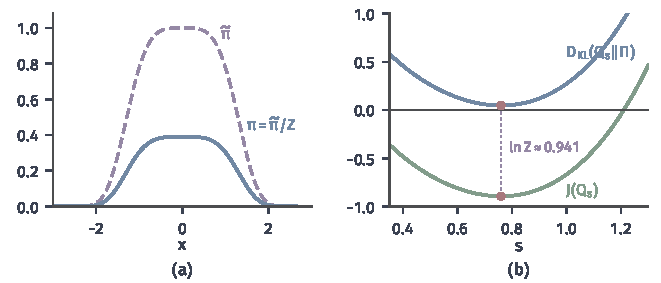
\includegraphics[width=112mm]{figures/07-probability/07-distribution-optimization/matplotlib/dapx-unnormalized/figure.pdf}
 \caption{未归一化目标。(a)$\widetilde{\pi}(x)=\mathrm{e}^{-x^{4}/4}$（紫色虚线）与归一化后的密度$\pi=\widetilde{\pi}/Z$（蓝），$Z\approx2.564$。(b)候选$Q_s=\mathcal{N}(0,s^{2})$：绿线是可计算的$J(Q_s)$，蓝线是$D_{\mathrm{KL}}(Q_s\Vert\Pi)$，两者相差常数$\ln Z\approx0.941$（紫色点线），在同一个$s^{*}=3^{-1/4}\approx0.760$处取最小值（红点）。}
 \label{fig:dapx-unnormalized}
\end{BookInlineFigure}

\paragraph{计算需求}
求$J(Q)$需要对候选$Q$求两个期望：$\ln q$与$\ln\widetilde{\pi}$。前者对高斯、乘积等候选通常有闭式；后者在本例中有闭式，一般情况下可以从$Q$抽样后取平均来估计，误差由第~\ref{chap:monte-carlo-integration-error}章分析。对目标$\Pi$只需要逐点计算$\widetilde{\pi}$，不需要$Z$，不需要从$\Pi$抽样，也不需要任何$\Pi$下的期望。这正是这个方向在目标难以计算时最常用的原因。

\subsection{按目标分布计算KL}
\label{sec:dapx-forward-kl}

第二个问题是
\begin{equation}
 \min_{Q\in\mathcal{Q}}D_{\mathrm{KL}}(\Pi\Vert Q)=\min_{Q\in\mathcal{Q}}\mathbb{E}_{\Pi}\Bigl[\ln\frac{\pi(X)}{q(X)}\Bigr] ,
 \label{eq:dapx-forward-problem}
\end{equation}
相应地常称为\term{正向KL散度}（forward KL divergence）的最小化。现在权重是$\pi$：目标常出现的地方，候选给的概率若太小就要付出代价。

\paragraph{有限的条件}
$D_{\mathrm{KL}}(\Pi\Vert Q)<\infty$要求$\Pi\ll Q$：候选必须覆盖目标有正概率的每个区域。只要漏掉一个这样的区域，KL就是$+\infty$。即使没有完全漏掉，覆盖不足也代价很重。取双峰目标
\begin{equation}
 \pi=0.7\,\mathcal{N}(-2,0.6^{2})+0.3\,\mathcal{N}(2,0.6^{2}) ,
 \label{eq:dapx-bimodal}
\end{equation}
候选$Q=\mathcal{N}(-2,0.6^{2})$只盖住左峰。数值积分给出
\[
 D_{\mathrm{KL}}(Q\Vert\Pi)\approx0.356,\qquad D_{\mathrm{KL}}(\Pi\Vert Q)\approx6.06 .
\]
按候选加权时，候选只看见左峰，在那里它的密度约是目标的$1/0.7$倍，代价约为$-\ln0.7\approx0.357$；按目标加权时，右峰有$0.3$的目标质量落在候选密度只有$\mathrm{e}^{-22}$量级的地方，峰顶处的对数比约为$21$，贡献了绝大部分代价。图~\ref{fig:dapx-weighting}(b)画出两个被积函数。

\begin{BookInlineFigure}
 \centering
 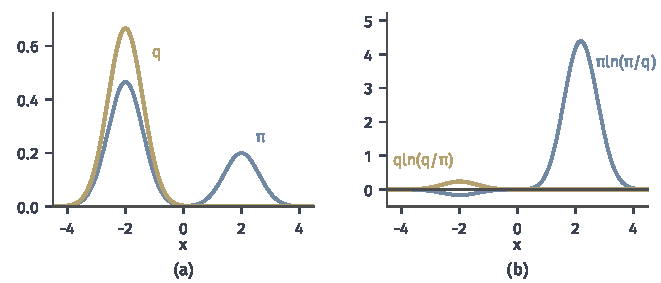
\includegraphics[width=112mm]{figures/07-probability/07-distribution-optimization/matplotlib/dapx-weighting/figure.pdf}
 \caption{两个方向的误差权重。(a)式~\eqref{eq:dapx-bimodal}的双峰目标（蓝）与只覆盖左峰的候选$\mathcal{N}(-2,0.6^{2})$（黄）。(b)被积函数：黄线$q\ln(q/\pi)$只在左峰附近有一个小鼓包，积分约$0.356$；蓝线$\pi\ln(\pi/q)$在右峰处高达$4$以上，积分约$6.06$。}
 \label{fig:dapx-weighting}
\end{BookInlineFigure}

\paragraph{与交叉熵的关系}
在离散情形，第~\ref{chap:information-measures}章已经证明，$H(\Pi)<\infty$时
\[
 D_{\mathrm{KL}}(\Pi\Vert Q)=H(\Pi,Q)-H(\Pi) .
\]
对一般的参考测度，同样的拆分需要两个积分分别有限：设$\mathbb{E}_{\Pi}\lvert\ln\pi(X)\rvert<\infty$与$\mathbb{E}_{\Pi}\lvert\ln q(X)\rvert<\infty$，则可以把对数比的期望拆成两项之差，
\begin{equation}
 D_{\mathrm{KL}}(\Pi\Vert Q)=\mathbb{E}_{\Pi}[\ln\pi(X)]-\mathbb{E}_{\Pi}[\ln q(X)] .
 \label{eq:dapx-forward-split}
\end{equation}
第一项与$Q$无关。于是在满足这两个条件的候选中，最小化正向KL等价于最大化$\mathbb{E}_{\Pi}[\ln q(X)]$，即使交叉熵最小。条件不能省：若$\mathbb{E}_{\Pi}\lvert\ln\pi\rvert=\infty$，式~\eqref{eq:dapx-forward-split}的右边可能是$\infty-\infty$，没有意义，只能回到对数比本身做比较。

式~\eqref{eq:dapx-forward-split}也说明了这个方向的计算需求：要算$\mathbb{E}_{\Pi}[\ln q(X)]$及其关于候选的变化，必须能对目标$\Pi$求期望，或者有从$\Pi$抽得的样本。候选再容易抽样也无济于事，因为平均是按$\Pi$做的。若手头只有未归一化的$\widetilde{\pi}$，这个方向反而无从下手。用样本平均代替$\mathbb{E}_{\Pi}$就是统计中的最大似然，它的统计性质属于卷八，本章只处理$\Pi$下的期望能够计算的情形。

\paragraph{指数族候选：矩匹配}
当候选集合是指数族时，正向KL的最优解有一个简单的刻画。设
\[
 q_{\bm{\theta}}(x)=h(x)\exp\bigl(\langle\bm{\theta},\bm{T}(x)\rangle-A(\bm{\theta})\bigr),\qquad \bm{\theta}\in\Theta ,
\]
是第~\ref{chap:distribution-families}章的正则指数族，$\Theta$是开的自然参数域。由那里的结论，$\bm{T}$在每个$q_{\bm{\theta}}$下各阶矩有限，并且对数配分函数的梯度是均值参数：
\[
 \nabla A(\bm{\theta})=\mathbb{E}_{q_{\bm{\theta}}}[\bm{T}(X)] .
\]
最小化$-\mathbb{E}_{\Pi}[\ln q_{\bm{\theta}}]$时，对$\bm{\theta}$求梯度得到$\nabla A(\bm{\theta})-\mathbb{E}_{\Pi}[\bm{T}]$。这提示最优候选应当与目标有相同的$\bm{T}$的期望。下面的定理把这个提示变成完整的结论，并且不需要拆分式~\eqref{eq:dapx-forward-split}所要求的熵条件。

\begin{theorem}[正向KL与矩匹配]
\label{thm:dapx-moment-matching}
设$\{q_{\bm{\theta}}:\bm{\theta}\in\Theta\}$是上述正则指数族，$\mathbb{E}_{\Pi}\lVert\bm{T}(X)\rVert_2<\infty$。设存在$\bm{\theta}^{*}\in\Theta$使
\begin{equation}
 \mathbb{E}_{q_{\bm{\theta}^{*}}}[\bm{T}(X)]=\mathbb{E}_{\Pi}[\bm{T}(X)] ,
 \label{eq:dapx-moment-match}
\end{equation}
并且$D_{\mathrm{KL}}(\Pi\Vert Q_{\bm{\theta}^{*}})<\infty$。则对每个$\bm{\theta}\in\Theta$，
\begin{equation}
 D_{\mathrm{KL}}(\Pi\Vert Q_{\bm{\theta}})=D_{\mathrm{KL}}(\Pi\Vert Q_{\bm{\theta}^{*}})+D_{\mathrm{KL}}(Q_{\bm{\theta}^{*}}\Vert Q_{\bm{\theta}}) .
 \label{eq:dapx-pythagoras}
\end{equation}
因此$Q_{\bm{\theta}^{*}}$是族内唯一使正向KL最小的分布。
\end{theorem}

\begin{proof}
族中各成员的密度在同一个集合$\{h>0\}$上为正，所以它们相互绝对连续。由$D_{\mathrm{KL}}(\Pi\Vert Q_{\bm{\theta}^{*}})<\infty$知$\Pi\ll Q_{\bm{\theta}^{*}}$，于是$\Pi\ll Q_{\bm{\theta}}$。在$\{h>0\}$上，由密度的链式法则，
\[
 \ln\frac{\pi}{q_{\bm{\theta}}}=\ln\frac{\pi}{q_{\bm{\theta}^{*}}}+\ln\frac{q_{\bm{\theta}^{*}}}{q_{\bm{\theta}}} .
\]
第二项是$\bm{T}$的仿射函数：
\[
 \ln\frac{q_{\bm{\theta}^{*}}(x)}{q_{\bm{\theta}}(x)}=\langle\bm{\theta}^{*}-\bm{\theta},\bm{T}(x)\rangle-A(\bm{\theta}^{*})+A(\bm{\theta}) .
\]
由$\mathbb{E}_{\Pi}\lVert\bm{T}\rVert_2<\infty$，它在$\Pi$下可积；第一项的期望是有限的$D_{\mathrm{KL}}(\Pi\Vert Q_{\bm{\theta}^{*}})$。两项都有有限期望，可以逐项取$\Pi$下的期望。第二项的期望用式~\eqref{eq:dapx-moment-match}换成$Q_{\bm{\theta}^{*}}$下的期望：
\[
 \langle\bm{\theta}^{*}-\bm{\theta},\mathbb{E}_{\Pi}[\bm{T}]\rangle-A(\bm{\theta}^{*})+A(\bm{\theta})
 =\mathbb{E}_{q_{\bm{\theta}^{*}}}\Bigl[\ln\frac{q_{\bm{\theta}^{*}}(X)}{q_{\bm{\theta}}(X)}\Bigr] .
\]
右边就是$D_{\mathrm{KL}}(Q_{\bm{\theta}^{*}}\Vert Q_{\bm{\theta}})$，这里$\bm{T}$在$Q_{\bm{\theta}^{*}}$下可积，因为$\bm{\theta}^{*}$在开的参数域内。两项相加得式~\eqref{eq:dapx-pythagoras}。由Gibbs不等式，第二项非负，且仅当$Q_{\bm{\theta}}=Q_{\bm{\theta}^{*}}$时为零，所以$Q_{\bm{\theta}^{*}}$是唯一的最小者。
\end{proof}

式~\eqref{eq:dapx-pythagoras}像勾股定理：从$\Pi$到族内任一点的“距离”，等于从$\Pi$到最优点的“距离”加上族内两点之间的“距离”。定理要求式~\eqref{eq:dapx-moment-match}有解。若$\mathbb{E}_{\Pi}[\bm{T}]$落在均值参数可取值集合的边界上，族内没有完全匹配的成员，最优解可能不存在；这和第~\ref{chap:distribution-selection}章矩匹配遇到的边界情形相同。

用这个定理可以直接写出几个最优候选。高斯族的$\bm{T}(x)=(x,x^{2})$，匹配均值和二阶矩，也就是匹配均值和方差。式~\eqref{eq:dapx-bimodal}的双峰目标均值为$0.7\cdot(-2)+0.3\cdot2=-0.8$，方差为
\[
 0.6^{2}+\bigl(0.7\cdot4+0.3\cdot4\bigr)-0.8^{2}=0.36+4-0.64=3.72 ,
\]
所以最优高斯候选是$\mathcal{N}(-0.8,3.72)$。$\operatorname{Exp}(1)$目标的最优高斯候选是$\mathcal{N}(1,1)$，此时正向KL为$\tfrac12\ln(2\pi)-\tfrac12\approx0.419$；而按候选加权的方向对它没有任何有限的候选。四次方目标关于原点对称，均值为零，二阶矩为
\[
 \mathbb{E}_{\Pi}[X^{2}]=\frac{2\,\Gamma(3/4)}{\Gamma(1/4)}\approx0.6760 ,
\]
所以最优高斯候选是$\mathcal{N}(0,0.6760)$。它比上一小节按候选加权得到的$\mathcal{N}(0,0.5774)$宽。

\subsection{KL方向的比较}
\label{sec:dapx-direction-compare}

两个方向都在同一个候选集合里挑选，都以同一个目标为准，结果为什么会不同？一个全部概率为正、只有三个状态的例子就足以说明。取目标与单参数候选族
\begin{equation}
 \Pi=\bigl(\tfrac35,\tfrac{3}{10},\tfrac{1}{10}\bigr),\qquad Q_t=(t,\ 1-2t,\ t),\quad 0<t<\tfrac12 .
 \label{eq:dapx-three-point}
\end{equation}
候选要求状态$1$和状态$3$概率相同，而目标在这两个状态上的概率是$0.6$与$0.1$，相差悬殊。候选只有一个自由度，它必须在“两端各给多少”上作出取舍。

\paragraph{按候选加权}
记$f(t)=D_{\mathrm{KL}}(Q_t\Vert\Pi)$。逐项写出：
\[
 f(t)=t\ln\frac{t}{0.6}+(1-2t)\ln\frac{1-2t}{0.3}+t\ln\frac{t}{0.1} .
\]
对$t$求导。每一项$u\ln(u/c)$对$u$的导数是$\ln(u/c)+1$，中间一项的$u=1-2t$还要乘以$-2$；常数$1$在三项中合计$1-2+1=0$，于是
\[
 f'(t)=\ln\frac{t}{0.6}+\ln\frac{t}{0.1}-2\ln\frac{1-2t}{0.3} .
\]
驻点方程比较的是对数概率比：
\begin{equation}
 \tfrac12\Bigl[\ln\frac{q(1)}{\pi(1)}+\ln\frac{q(3)}{\pi(3)}\Bigr]=\ln\frac{q(2)}{\pi(2)} .
 \label{eq:dapx-reverse-stationary}
\end{equation}
两端状态上对数比的平均，要等于中间状态的对数比。

把式~\eqref{eq:dapx-reverse-stationary}写成$t^{2}/(0.6\cdot0.1)=(1-2t)^{2}/0.3^{2}$，取正的平方根，
\[
 \frac{t}{1-2t}=\frac{\sqrt{0.06}}{0.3}=\sqrt{\tfrac23} .
\]
解出
\[
 t_{\mathrm{r}}=\frac{\sqrt{2/3}}{1+2\sqrt{2/3}}=\frac{4-\sqrt6}{5}\approx0.3101 .
\]
又$f''(t)=2/t+4/(1-2t)>0$，$f$是严格凸函数，这个驻点是唯一的最小点。可以看出，按候选加权时两端共享的概率由$\pi(1)$与$\pi(3)$的几何平均$\sqrt{0.06}\approx0.245$决定，再与$\pi(2)=0.3$一起归一化。

\paragraph{按目标加权}
记$g(t)=D_{\mathrm{KL}}(\Pi\Vert Q_t)$。与$t$有关的只有交叉熵部分：
\[
 g(t)=\sum_{k}\pi(k)\ln\pi(k)-0.7\ln t-0.3\ln(1-2t) .
\]
求导得
\[
 g'(t)=-\frac{0.7}{t}+\frac{0.6}{1-2t} .
\]
驻点方程比较的是概率比的倒数，即目标与候选之比：
\begin{equation}
 \tfrac12\Bigl[\frac{\pi(1)}{q(1)}+\frac{\pi(3)}{q(3)}\Bigr]=\frac{\pi(2)}{q(2)} .
 \label{eq:dapx-forward-stationary}
\end{equation}
代入数值，驻点方程是$0.7(1-2t)=0.6t$，解得
\[
 t_{\mathrm{f}}=0.35 .
\]
又$g''(t)=0.7/t^{2}+1.2/(1-2t)^{2}>0$，这也是唯一的最小点。此时两端各得$\pi(1)$与$\pi(3)$的算术平均$0.35$，中间状态的$0.3$与目标完全相同。这正是定理~\ref{thm:dapx-moment-matching}的结论：$Q_t$是统计量$T=\mathbf{1}_{\{X\neq2\}}$生成的指数族，正向KL的最优解匹配$\mathbb{E}[T]=\Pi(X\neq2)=0.7$。

\paragraph{两个解的比较}
两个最优候选为
\[
 Q_{t_{\mathrm{r}}}\approx(0.310,\ 0.380,\ 0.310),\qquad Q_{t_{\mathrm{f}}}=(0.35,\ 0.30,\ 0.35) .
\]
把每个解放到另一个方向上评价，各自都不是最优：
\[
 \begin{aligned}
 D_{\mathrm{KL}}(Q_{t_{\mathrm{r}}}\Vert\Pi)&\approx0.2359, & D_{\mathrm{KL}}(Q_{t_{\mathrm{f}}}\Vert\Pi)&\approx0.2498,\\
 D_{\mathrm{KL}}(\Pi\Vert Q_{t_{\mathrm{r}}})&\approx0.2121, & D_{\mathrm{KL}}(\Pi\Vert Q_{t_{\mathrm{f}}})&\approx0.1981 .
 \end{aligned}
\]
差别的来源在状态$3$与状态$1$。状态$3$的目标概率只有$0.1$，候选给它$t\geq0.31$：按候选加权时这一项是$t\ln(t/0.1)$，权重大、对数比也大，所以$t$被压低，多出的概率转给中间状态。状态$1$的目标概率是$0.6$，候选只给$t\leq0.35$：按目标加权时这一项是$0.6\ln(0.6/t)$，权重是$0.6$，所以$t$被抬高。

\begin{BookInlineFigure}
 \centering
 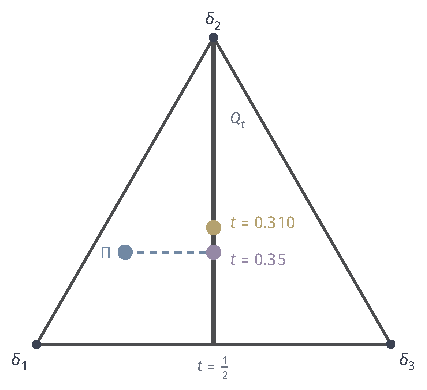
\includegraphics[width=72mm]{figures/07-probability/07-distribution-optimization/tikz/dapx-simplex-segment/figure.pdf}
 \caption{三状态概率表组成的三角形，顶点$\delta_k$是集中在状态$k$的分布，一点到三边的远近给出三个概率。蓝点是目标$\Pi=(0.6,0.3,0.1)$，深灰粗线是候选族$Q_t$（从$\delta_2$到底边中点）。黄点是按候选加权的最优解$t=0.310$，紫点是按目标加权的最优解$t=0.35$，它与$\Pi$等高，即中间状态的概率同为$0.3$。}
 \label{fig:dapx-simplex-segment}
\end{BookInlineFigure}

图~\ref{fig:dapx-simplex-segment}把这件事放在概率单纯形里：候选族是一条线段，目标在线段之外，两个方向在线段上选了不同的点。图~\ref{fig:dapx-three-point}画出两条目标曲线和三个分布的概率。两条曲线都是凸的，最低点相距$0.04$；概率图中，黄色候选把多出的概率放在中间状态，紫色候选保持中间状态与目标一致。

\begin{BookInlineFigure}
 \centering
 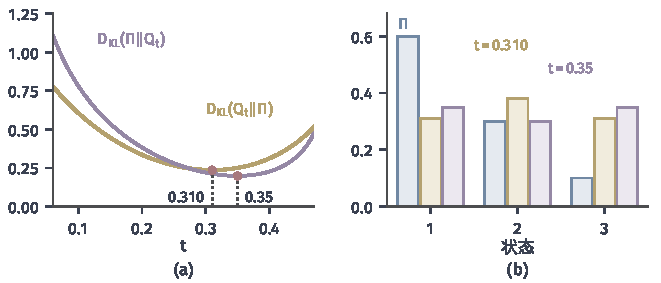
\includegraphics[width=112mm]{figures/07-probability/07-distribution-optimization/matplotlib/dapx-three-point/figure.pdf}
 \caption{三状态例子的两个方向。(a)$D_{\mathrm{KL}}(Q_t\Vert\Pi)$（黄）与$D_{\mathrm{KL}}(\Pi\Vert Q_t)$（紫）随$t$的变化，红点是最小点$t=0.310$与$t=0.35$。(b)目标$\Pi$（蓝）与两个最优候选（黄：$t=0.310$；紫：$t=0.35$）在三个状态上的概率。}
 \label{fig:dapx-three-point}
\end{BookInlineFigure}

\paragraph{择峰与覆盖}
目标有几个分离的峰而候选只有一个峰时，两个方向的差别最明显。式~\eqref{eq:dapx-bimodal}的双峰目标用高斯族逼近：按目标加权的最优解是矩匹配的$\mathcal{N}(-0.8,3.72)$，它横跨两个峰，在两峰之间目标几乎没有质量的地方放了很多概率，KL约为$0.558$；按候选加权的目标函数有两个局部最小点，分别贴住一个峰，值约为$0.356$与$1.202$，接近$-\ln0.7$与$-\ln0.3$。图~\ref{fig:dapx-bimodal-fits}(b)对每个均值$m$先把$s$取到最优，画出两个目标随$m$的变化。

\begin{BookInlineFigure}
 \centering
 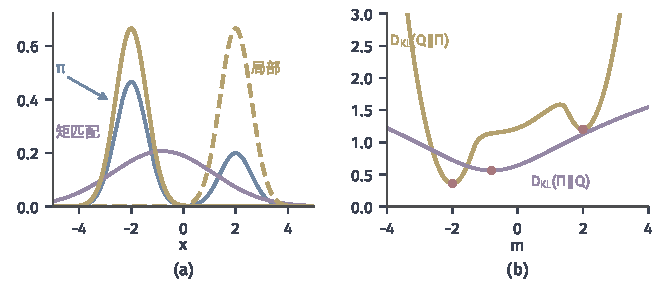
\includegraphics[width=112mm]{figures/07-probability/07-distribution-optimization/matplotlib/dapx-bimodal-fits/figure.pdf}
 \caption{用单个高斯逼近双峰目标。(a)目标（蓝）；按目标加权的最优解$\mathcal{N}(-0.8,3.72)$（紫，矩匹配）；按候选加权的两个局部最优解$\mathcal{N}(-2,0.6^{2})$（黄实线）与$\mathcal{N}(2,0.6^{2})$（黄虚线）。(b)固定均值$m$、把标准差$s$取到最优后的目标值：黄线是$D_{\mathrm{KL}}(Q\Vert\Pi)$，在$m=\pm2$附近各有一个局部最小（$0.356$与$1.202$）；紫线是$D_{\mathrm{KL}}(\Pi\Vert Q)$，只有一个最小点$m=-0.8$（$0.558$）。}
 \label{fig:dapx-bimodal-fits}
\end{BookInlineFigure}

按候选加权的方向倾向于选中目标的一个峰而忽略其他峰，称为\term{择峰}（mode seeking）；按目标加权的方向倾向于把目标所有有质量的区域都盖住，称为\term{质量覆盖}（mass covering）。这两个说法描述的是倾向，不是定理，是否出现要看目标与候选集合的具体形状。三状态例子里没有分离的峰，两个最优解都把正概率给了每个状态，按候选加权的解也没有“择”出哪一个状态，只是把概率从小概率的一端挪到了中间。能下结论的只有本节算出的这些事实：权重来自哪个分布，支持条件落在哪一边，驻点方程比较的是对数比还是比值本身。
